\chapter{隨機變數與機率分布}
    在前一章中，我們討論了機率的定義，以及如何利用機率來量化我們所關心之事件的可能性。舉例來說，如果我們做一個「丟兩枚銅板」的隨機實驗，我們可以針對銅板出現的正反面來定義事件，例如「一正一反」、「兩枚正反面相同」，並為這些事件賦予對應的機率。同樣地，我們也可以做一個「抽兩次撲克牌」的隨機實驗，並定義「一紅一黑」、「兩次抽牌的紅黑相同」的事件，這些事件也會有相應的機率。注意到，雖然這兩個實驗的實際內容不同，但它們實驗結果都是兩個二元的出象，因此機率結構有很高度的相似性。為了更好地描述這個底層的機率結構並進行進一步的推論，我們需要引入隨機變數的概念，並了解如何用機率分布描述隨機變數的機率結構，並從機率分布出發擷取出隨機變數的重要特徵，例如期望值、變異數等等，以輔助未來的統計推論。
    
\begin{introduction}[第 \thechapter 章學習目標]{1}
    \item 了解隨機變數的概念
    \item 了解如何描述離散與連續隨機變數的機率分布
    \item 隨機變數期望值與變異數的計算
    \item 常見離散分布的統計性質
    \item 常態分布的性質與 z 轉換
\end{introduction}

\section{隨機變數}

    以數學語言來說，隨機變數 (random variable) 的正式定義是「樣本空間上的一個可測函數」。這個定義看似艱深，但其本質是將實驗的可能結果對應到數字，以便於我們進行運算與處理。舉例來說，拋硬幣的結果不是正面就是反面，因此我們可以定義一個隨機變數 $X$ 來代表拋硬幣的未知結果（通常我們會以大寫字母表示隨機變數），並將正面編碼為 $1$、反面編碼為 $0$。同樣地，如果我們抽撲克牌並觀察其為紅色或黑色，我們同樣可以定義結果為另一個隨機變數 $Y$，並將紅色編碼為 $1$、黑色編碼為 $0$。

    \medskip
    
    以上的例子有兩點值得注意：第一，數值（$1$/$0$）與樣本空間（正面/反面、紅色/黑色）的對應關係並沒有硬性規定，因此把反面編碼為 $1$、正面編碼為 $0$ 仍然是有效的。第二，隨機變數仍是一個隨機的量，因此即使隨機變數 $X$ 的可能取值為 $1$ 或 $0$，它並\textbf{不等於} $1$ 或 $0$ 中的任何一個。唯有在我們執行隨機實驗（即拋硬幣）之後，才能根據實驗結果獲得 $X$ 的一個實現值 (realized value) 或觀察值 (observed value)。我們可以將隨機變數 $X$ 想像成一台轉輪有 $0$ 和 $1$ 的老虎機。當轉輪停止時，我們得到的是 $X$ 的一個實現值。但當我們談論 $X$ 本身時，我們指的是整台機器，其轉輪仍在轉動的狀態。因此，描述 $X$ 統計性質的方式，就是描述其所有可能結果各自發生的機率。這些機率合稱為隨機變數 $X$ 的機率分布 (probability distribution)（有時簡稱為分布 (distribution)）。描述隨機變數機率分布的方式，取決於其可能取值是離散 (discrete) 還是連續 (continuous) 的，因此在以下各節中，我們將分別探討離散型與連續型隨機變數。
    
\section{離散型機率分布}

    當隨機變數的取值是可數的 (countable)，我們可以將各取值出現的機率做一個表列，就能完整描述其機率分布。這種隨機變數被稱為\textit{離散型隨機變數} (discrete random variable)，其分布則被稱為\textit{離散型機率分布} (discrete probability distribution)。舉例來說，在前面擲銅板的例子中，若欲描述 $X$ 的分布，我們可以把兩種取值出現的機率做一個表列，例如 $\PP(X = 1) = 0.8;\; \PP(X = 0) = 0.2$。為了更加簡化，我們定義 $X$ 的機率質量函數 (probability mass function, 常用小寫 $f$ 表示)為：
    \smallskip
    \[f_X(x) := \PP(X = x)\]
    \smallskip
    如此一來， $X$ 的機率質量函數取值如下
    \smallskip
    \[f_X(x) = \left\{\begin{array}{rl}
            0.8, & x = 1\\
            0.2, & x = 0\\
            0, & \text{其他}
        \end{array}\right.\]
    \smallskip
    這個函數包含了 $X$ 所有不確定性的資訊，因此機率質量函數就像隨機變數的指紋一樣，可以\textbf{完全}定義隨機變數的分布。注意到由於總機率等於 $1$，所以機率質量函數裡面的各取值對應的機率總和必然等於 1 ($0.8+0.2=1$)。如果另一個隨機變數 $W$ 的可能取值是所有的非負整數 $0, 1, 2, ...$，那麼只要知道 $f_Y(0), f_Y(1), f_Y(2), ...$ 的數值，就可以完整描述 $Y$ 的分布，且必須有$f_Y(0)+f_Y(1)+f_Y(2)+... = \sum_i^\infty f_Y(i) = 1$。
    
    除了機率質量函數以外，另一個常用的函數是\textit{累積分配函數} (cumulative distribution function, 常用大寫 $F$ 來表示)，其定義為：
    \smallskip
    \[F_X(x) := \PP(X \le x)\]
    \smallskip
    例如上述銅板的例子中，我們就有
    \smallskip
    \[F_X(x) = \left\{\begin{array}{rl}
        0, & x < 0\\
        0.2, & x < 1\\
        1, & x \ge 1
    \end{array}\right.\]
    
    為了對隨機變數做進一步瞭解，我們可以把隨機變數的機率分布看作是一個母體，而隨機變數的取值就是從母體抽樣的結果。因此，如果我們知道機率分布的敘述性參數，例如作為位置參數的平均值、和作為分散參數的變異數和標準差，那麼就知道相對應隨機變數的取值中心以及分散程度。隨機變數機率分布的平均值也被稱作隨機變數的\textit{期望值} (expected value)，其計算方法如下（其中 $\mathcal{X}$ 是 隨機變數 $X$ 所有可能取值的集合，也被稱為 $X$ 的\textit{支撐集} (support)）。
    \smallskip
    \[\EE(X) = \sum_{x\in\mathcal{X}} x \cdot f_X(x)\]
    \smallskip
    可以看到期望值的計算方法，是把每個可能的取值依出現機率做\textbf{加權平均}。例如前面擲銅板的例子中，$X$ 的期望值就是 $\EE(X) = 1 \times 0.8 + 0 \times 0.2 = 0.8$。同理，隨機變數機率分布的變異數和標準差計算方法為
    \begin{align*}
        var(X) &= \sum_{x\in\mathcal{X}} (x-\EE(X))^2 \cdot f_X(x)\\
        sd(X) &= \sqrt{var(X)}
    \end{align*}
    這裡 $var(X)$ 的算法也是加權平均，但是要平均的是取值和期望值的距離平方，符合我們在敘述性統計時的作法。不過，上述的計算過程通常比較繁瑣，所以我們會使用另外一個計算公式（注意到 $\EE(X)$ 是一個數字，和加總符號使用的 $x$ 無關，所以在很多地方可以提出加總符號外）：
    \begin{align*}
        var(X) &= \sum_{x\in\mathcal{X}} (x-\EE(X))^2 \cdot f_X(x)\\
        &= \sum_{x\in\mathcal{X}} [x^2 - 2x\EE(X) + (\EE(X))^2] \cdot f_X(x)\\
        &= \Big[\sum_{x\in\mathcal{X}} x^2 \cdot f_X(x)\Big] - \Big[\sum_{x\in\mathcal{X}} 2x\EE(X) \cdot f_X(x)\Big] + \Big[\sum_{x\in\mathcal{X}} (\EE(X))^2 \cdot f_X(x)\Big]\\
        &= \Big[\sum_{x\in\mathcal{X}} x^2 \cdot f_X(x)\Big] - 2\EE(X)\Big[\sum_{x\in\mathcal{X}} x \cdot f_X(x)\Big] + (\EE(X))^2\Big[\sum_{x\in\mathcal{X}} f_X(x)\Big]\\
        &= \Big[\sum_{x\in\mathcal{X}} x^2 \cdot f_X(x)\Big] - 2\EE(X)\EE(X) + (\EE(X))^2\\
        &= \EE(X^2) - (\EE(X))^2
    \end{align*}
    倒數第二行的第一項是把每個可能取值的平方做加權平均，因此在符號上寫作 $\EE(X^2)$，也就是 $X^2$ 的期望值。前面擲銅板的例子中，$X^2$ 的期望值是 $\EE(X^2)=1^2 \times 0.8 + 0^2 \times 0.2 = 0.8$，所以 $X$ 的變異數為 $\EE(X^2) - (\EE(X))^2 = 0.8-0.8^2 = 0.16$，而 $X$ 的標準差則為 $\sqrt{0.16} = 0.4$。

    當我們對隨機變數作線性轉換的時候，它的期望值和變異數的變化就如同我們在敘述性統計所提到的：
    \begin{align*}
        \EE(aX+b) &= a\EE(X) + b\\
        var(aX+b) &= a^2 var(X)
    \end{align*}
    而當我們對兩個隨機變數 $X, Y$ 做相加減時，期望值也會相加減
    \smallskip
    \[\EE(X \pm Y) = \EE(X) \pm \EE(Y)\]
    \smallskip
    如果這兩個隨機變數還互相\textbf{獨立}，那麼變異數則會相加
    \smallskip
    \[var(X \pm Y) = var(X) + var(Y)\]
    
    以下我們介紹幾個生物醫學統計中常用到的離散分布以及其性質：

\subsection{白努利分布}

    前面我們提到擲銅板的例子中，我們根據 $X=0$ 和 $X=1$ 的機率寫出隨機變數 $X$ 的機率質量函數。一般性地來說，如果隨機變數 $X$ 僅能取值 $0$ 或 $1$，而且把 $X=1$ 的機率寫為 $p$，那麼由於機率總和為 1，$X=0$ 的機率就必然是 $1-p$。根據這樣的設定所得的機率質量函數為
    \smallskip
    \[f_X(x) = \left\{\begin{array}{rl}
        p, & x = 1\\
        1-p, & x = 0
    \end{array}\right.\]
    \smallskip
    這個機率質量函數作圖如圖\ref{fig:bernoulli}，其所對應的分布被稱為\textit{白努利分布} (Bernoulli distribution)。白努利分佈有一個參數 $p$，代表隨機變數取值為 $1$ 的機率。的當一個隨機變數 $X$ 服從參數為 $p$ 的白努利分布，我們會寫作
    \smallskip
    \[X \sim Bernoulli(p)\]

    \begin{figure}[htbp]
      \centering
      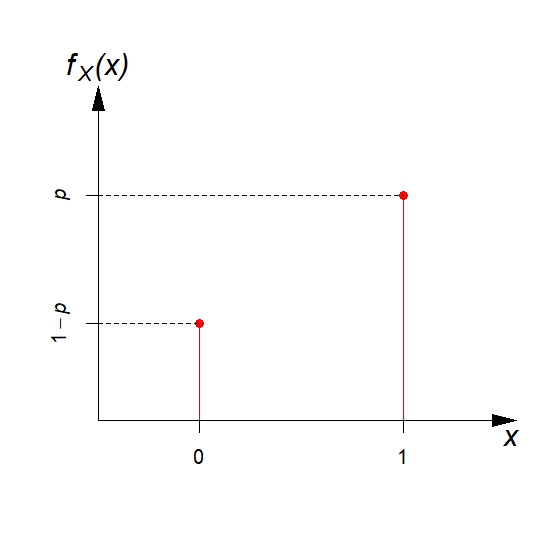
\includegraphics[width=0.5\textwidth]{figures/04-Random_variable_probability_distribution/Bernoulli.jpeg}
      \caption{白努利分佈的機率質量函數}
      \label{fig:bernoulli}
    \end{figure}
    
    白努利分布的命名來自於瑞士數學家 Jacob Bernoulli（1654-1705），是最簡單也最常用的的離散型機率分布。所有的二元變數，舉凡性別的男女、疾病發病與否、是否接受治療、收縮壓是否於140毫米汞柱以上，將有興趣的類別編碼為 1，另一個類別編碼為 0 後，其分布均可用白努利分布來描述，其中參數 $p$ 為類別為 $1$ 的機率。簡單計算白努利分布之期望值和變異數可得到期望值為 $p$，變異數為 $p(1-p)$。

    \medskip

    \begin{custom}{動手作}
        用前述期望值和變異數的定義推導出白努利分布的期望值和變異數。
    \end{custom}
    
    \medskip\noindent\framebox[\textwidth]{\rule{0pt}{180pt}}
    
    \medskip

    \begin{custom}{動動腦}
        我們知道變異數是分佈取值分散性的度量。根據這個想法，白努利分布的變異數應該在 $p$ 取值多少時為最小、$p$ 取值多少時為最大？剛剛我們算出分布的變異數為 $p(1-p)$，這個結果是否符合你的預測？
    \end{custom}
    
    \medskip\noindent\framebox[\textwidth]{\rule{0pt}{150pt}}

\subsection{二項式分布}
    我們剛剛提到的白努利分布對應到的是擲一次銅板並觀察是否為正面。如果我們擲了同一枚銅板多次，然後再計算正面的次數，對應到的就是\textit{二項式分佈} (binomial distribution)。假設我們擲了 3 次銅板，每次擲銅板時正面機會均為 0.8，那麼有 2 次正面的情況共有 3 種：第一、二次正面、第三次反面；第一、三次正面、第二次反面；第二、三次正面、第一次反面。情況的總數可以用高中的組合數來計算，也就是$C^3_2$或寫做$\binom{3}{2}$。每種情況都是兩次正面、一次反面，所以機率都是 $0.8^2 \cdot 0.2$。因此，總共出現 2 次正面的機率可以寫作 $\binom{3}{2} 0.8^2 \cdot 0.2 = 0.384$。按照上述的算法，如果我們把 $X$ 令為投擲 $n$ 次銅板，每次正面機會為 $p$ 時，出現正面次數的隨機變數，那麼 $X$ 的機率質量函數可寫為：
    \medskip
    \[f_X(x) = \binom{n}{x} p^x (1-p)^{n-x},\qquad x \in \{0,1,2,...,n\}\]
    \medskip
    此時我們稱隨機變數 $X$ 服從次數參數為 $n$，機率參數為 $p$ 的二項式分布，寫作
    \smallskip
    \[X \sim Binomial(n,p)\]
    
    \begin{figure}[htbp]
      \centering
      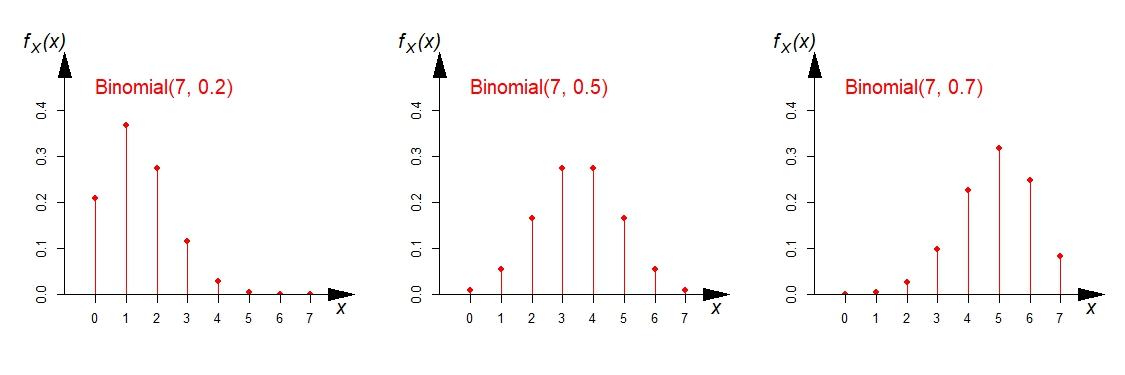
\includegraphics[width=\textwidth]{figures/04-Random_variable_probability_distribution/Binomial.jpeg}
      \caption{二項分佈的機率質量函數}
      \label{fig:binomial}
    \end{figure}
    
    二項式分佈的偏度隨著機參數率 $p$ 的不同而可能為左偏、對稱或右偏。如圖\ref{fig:binomial}繪製的機率質量函數所示，當 $p<0.5$ 時，二項式分佈呈現右偏；當 $p>0.5$ 時，二項式分佈呈現左偏；當 $p=0.5$ 時，二項式分佈為左右對稱。

    \medskip

    二項式分佈的期望值和變異數如果要從機率質量函數去推導，會需要相當麻煩的代數計算。但我們可以想像，二項式分佈所代表的銅板正面總次數，可以視為每次擲銅板時的正面次數（非 1 即 0）相加。如果 $X_1, X_2, ..., X_n$ 代表每次擲銅板正面與否，那麼他們都應該服從機率參數為 $p$ 的白努利分佈，而我們最終關心的正面總次數 $X = X_1 + X_2 + ... + X_n$。由於每次擲銅板的結果都是獨立的，所以根據我們前面提到有關期望值和變異數的性質：
    \begin{align*}
        \EE(X) &= \EE(X_1 + X_2 + ... + X_n)&\\
        &= \EE(X_1) + \EE(X_2) + ... + \EE(X_n) &\text{（相加的期望值等於期望值相加）}\\
        &= p + p + ... + p&\text{（每次擲銅板都服從} Bernoulli(p)\text{）}\\
        &= np&\\
        var(X) &= var(X_1 + X_2 + ... + X_n)&\\
        &= var(X_1) + var(X_2) + ... + var(X_n) &\text{（獨立隨機變數相加的變異數等於變異數相加}\\
        &= p(1-p) + p(1-p) + ... + p(1-p)&\text{（每次擲銅板都服從} Bernoulli(p)\text{）}\\
        &= np(1-p)&
    \end{align*}

    注意到這裡我們雖然是用擲銅板的正面次數來導出二項式分佈，但實際上二項式分佈可以用來描述一群樣本中，任意二元標籤的觀察總數。例如，如果抽樣 $n$ 位肺腺癌第三期的病患並統計三個月內復發的人數 $X$，那麼 $X$ 也會服從二項式分佈，其中次數參數為 $n$，機率參數 $p$ 則為「所有肺腺癌第三期的病患的三個月內復發機率」。
    
\subsection{卜瓦松分布}
    前面我們提到，如果我們有興趣的離散型隨機變數是二元的，可以用白努利分布描述；如果該離散型隨機變數可以被解釋為一群樣本中，二元標籤的觀察總數，則可以用二項式分布描述。但生物醫學中還有一種常見離散型資料：次數資料。這種離散型資料可以轉化為一段時間內事件發生的次數，例如三個月內的癲癇發作次數、每年嚴重藥物過敏的發生次數、胰臟癌每年新發個案等等。其可能取值為非負整數，最大可能取值為無上限、或可近似為無上限。

    \begin{figure}[htbp]
        \centering
        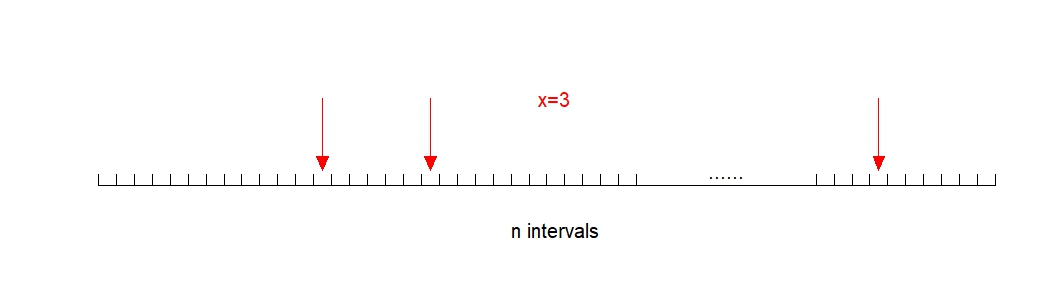
\includegraphics[width=\textwidth]{figures/04-Random_variable_probability_distribution/Poisson_exp.jpeg}
        \caption{以二項分布近似卜瓦松分佈}
        \label{fig:poisson_exp}
    \end{figure}

    描述次數資料最常用的分布是\textit{卜瓦松分布} (Poisson distribution)，其命名來自於法國數學家 Siméon Poisson（1781-1840）。假設事件的發生滿足以下條件：(1) 發生事件之間為獨立 (2) 發生事件的頻率不隨時間點而改變 (3) 同一個時間點不會發生兩次以上的事件。那麼如圖\ref{fig:poisson_exp}所示，我們可以把追蹤的時間切成 $n$ 等分。根據上述的前兩個條件，每一等分發生事件的機率都相同且彼此獨立，而且在 $n$ 越來越大的情況下，根據第三個條件，每一個等分最多只會發生一件事件，且發生事件的機率可寫為 $\lambda/n$，其中 $\lambda$ 為在整段時間內預期發生事件的次數。整條時間線可以被看成作了 $n$ 次互相獨立、成功機率為 $\lambda/n$ 的實驗，而我們關心的是成功的總次數 $X$。在這個近似的框架下，$X$ 應該服從二項式分配，其機率質量函數可寫做
    \smallskip
    \begin{align*}
        f_X(x) = \binom{n}{x} \Big(\frac{\lambda}{n}\Big)^x\Big(1-\frac{\lambda}{n}\Big)^{n-x} &= \frac{n (n-1)...(n-x+1)}{x!}\frac{\lambda^x}{n^x}\Big(1-\frac{\lambda}{n}\Big)^n\Big(1-\frac{\lambda}{n}\Big)^{-x}\\
        &= \frac{n (n-1)...(n-x+1)}{n^x} \Big(1-\frac{\lambda}{n}\Big)^{-x} \frac{\lambda^x}{x!} \Big(1-\frac{\lambda}{n}\Big)^n
    \end{align*}
    
    \smallskip
    \noindent 當切的等分數 $n$ 趨近於無窮大時，前兩項都會趨近於 $1$，而最後一項則會趨近於 $e^{-\lambda}$（$e$是自然對數的底，約 2.718）。因此，卜瓦松分佈的機率質量函數為
    \smallskip
    \[f_X(x) = \frac{\lambda^x e^{-\lambda}}{x!}, \qquad x \in \{0,1,2,3,...\}\]
    \smallskip
    此時我們稱隨機變數 $X$ 服從速率參數 (rate parameter) $\lambda$ 的卜瓦松分布，寫作
    \smallskip
    \[X \sim Poisson(\lambda)\]

    卜瓦松分布是一個右偏分布，如圖\ref{fig:poisson}所示，但偏度會隨著 $\lambda$ 增加而降低。根據前面用 $Binomial(n, \lambda/n)$ 二項式分佈的近似，卜瓦松分布的期望值為 $n \cdot (\lambda/n) = \lambda$。變異數則可用 $n \cdot (\lambda/n) \cdot (1- \lambda/n) = \lambda \cdot (1- \lambda/n)$ 近似，在 $n$ 趨近於無窮大時亦趨近至 $\lambda$。由此可知，卜瓦松分佈的特性為期望值和變異數相等。

    \begin{figure}[htbp]
        \centering
        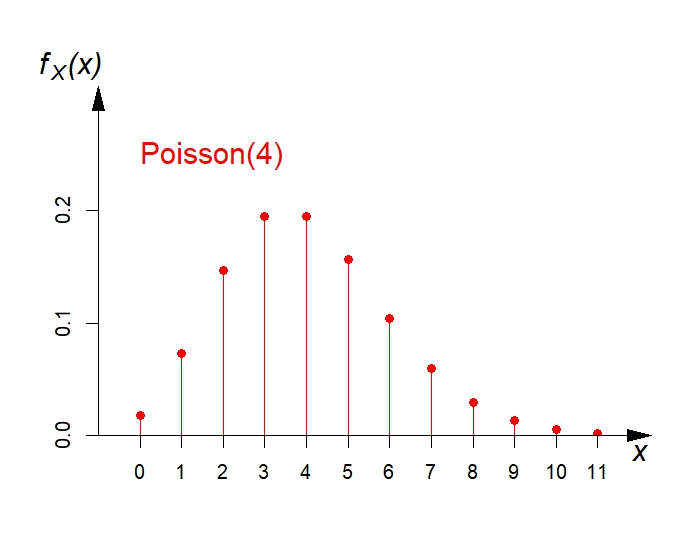
\includegraphics[width=0.7\textwidth]{figures/04-Random_variable_probability_distribution/Poisson.jpeg}
        \caption{卜瓦松分佈的機率質量函數}
        \label{fig:poisson}
    \end{figure}

    \pagebreak

    \begin{custom}{動手作}
        根據一項大型世代研究，45 歲以上氣喘患者的平均急性發作率為一年 0.22 次。若氣喘發作的次數可用卜瓦松分配描述，那麼如何計算一位 45 歲以上氣喘患者在半年內發作兩次以上的機率？
    \end{custom}
    
    \medskip\noindent\framebox[\textwidth]{\rule{0pt}{220pt}}

    \bigskip

    \begin{custom}{動動腦}
        我們前面提到卜瓦松分佈的特性是期望值和變異數相等。如果我們抽樣的樣本並不「純粹」，而是來自多個速率參數不同的母體，那麼我們應該預期樣本變異數和樣本期望值的關係為何？
    \end{custom}

    \medskip\noindent\framebox[\textwidth]{\rule{0pt}{180pt}}


    \bigskip

    最後，我們用表\ref{tab:discrete_distribution}來總結生物醫學統計常用的離散型機率分布。

    \bigskip
    
    \begin{table}[htbp]
        \begin{center}
            \begin{tabular}{cccc}
                \toprule
                分布名稱 & 參數 & 期望值 & 變異數\\
                \hline
                白努利 (Bernoulli) 分布 & 機率參數 $p$ & $p$ & $p(1-p)$\\
                二項式 (Binomial)分布 & 次數參數 $n$；機率參數 $p$ & $np$ & $np(1-p)$\\
                卜瓦松 (Poisson) 分布 & 速率參數 $\lambda$ & $\lambda$ & $\lambda$\\
                \bottomrule
            \end{tabular}
            \caption{生物醫學統計常用的離散型機率分布\label{tab:discrete_distribution}}
        \end{center}
    \end{table}
    
\section{連續型機率分布}

    前面我們提到，當隨機變數的可能取值可數 (countable)，就適合用離散型機率分布來描述，而且取得機率質量函數就完全決定了機率分布。然而，還有一類隨機變數的取值是連續而不可數的。舉例來說，如果我們在 Excel 裡輸入 \textit{RAND()} 函數，程式會隨機吐出一個 0 到 1 之間的亂數。我們把這個吐出的亂數記作隨機變數 $X$。如果小數位數無限增多，那麼從 0 到 1 之間的所有實數都是 $X$ 可能的取值，因此 $X$ 不是離散型的隨機變數，而是連續型的隨機變數，其所服從的也是一個\textit{連續型機率分布} (continuous probability distribution)。

    \medskip

    在連續型機率分布中，機率質量函數是沒有意義的。舉例而言，上述的 $X$ 若有機率質量函數 $f_X(x)$，則 $f_X(0.5)$ 應該代表 $X = 0.5$ 的機率。然而，$X$ 的取值是連續的，所以雖然 $X$ 可以取值 0.5，但 $X = 0.5$ 的機率等於零。事實上，$X$ 等於任何一個數的機率都等於零，所以 $X$ 的機率質量函數無法提供任何資訊。取而代之的是\textit{機率密度函數} (probability density function)，如圖\ref{fig:uniform}所示。機率密度函數\textbf{曲線下的面積}代表取值區間出現的機率，例如圖中藍色的曲線下面積等於 $(0.7-0.4) \times 1 = 0.3$，代表 $X$ 取值於 0.4 到 0.7 之間的機率 $\PP(0.4 \le X \le 0.7) = 0.3$。我們也可以看到，如果區間取 「0.5 到 0.5 之間」，那麼曲線下就沒有面積，也就隱含著 $\PP(0.5 \le X \le 0.5) = \PP(X=0.5) = 0$，和我們前述單點機率等於零的結論相符。由於曲線下的面積才是機率，機率密度函數的實際取值並非機率而是\textit{機率密度} (probability density)，用來度量隨機變數。也因此，雖然機率質量函數的取值不能超過 1（否則會違反總機率等於一的規則），但機率密度函數的取值卻可以超過 1，只要任何曲線下面積都不超過 1 即可。總機率等於一的規則在機率密度函數的體現，就是曲線下的總面積要等於一，寫成數學式就必須要動用到積分：
    \smallskip
    \[\int_{-\infty}^{\infty} f_X(x) dx = 1\]
    \smallskip
    讀者可以依此來檢查圖\ref{fig:uniform}的機率密度函數是否有符合總機率等於一的規則。
    \begin{figure}[htbp]
        \centering
        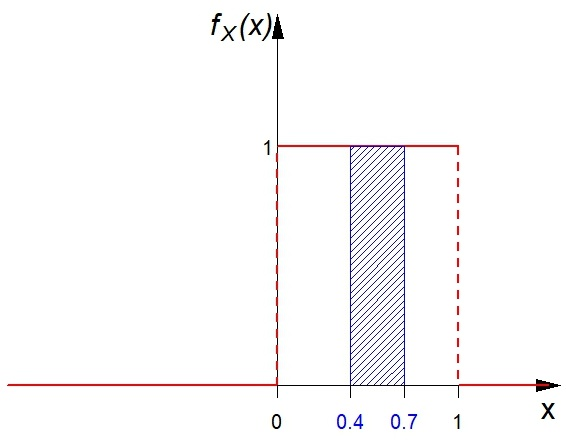
\includegraphics[width=0.65\textwidth]{figures/04-Random_variable_probability_distribution/Uniform.jpeg}
        \caption{標準均一分布的機率密度函數}
        \label{fig:uniform}
    \end{figure}

    在離散型機率分布中，我們提到期望值的算法是將各取值以出現機率作加權平均，而變異數則是將「各取值與期望值距離的平方」以出現機率作加權平均。在連續型機率分布中，由於取值是連續的，我們需要將前面的定義用積分作小小的修正：
    \smallskip
    \[\EE(X) = \int_{-\infty}^{\infty} x f_X(x) dx\]
    \[var(X) = \int_{-\infty}^{\infty} (x-\EE(X))^2 f_X(x) dx\]
    \smallskip
    如果想要用 $var(X) = \EE(X^2) - (\EE(X))^2$ 來計算變異數，則需要用到
    \[\EE(X^2) = \int_{-\infty}^{\infty} x^2 f_X(x) dx\]

    \medskip

    另外，我們在離散型機率分布中提到的累積分配函數，在連續型機率分佈中仍然適用。其計算方式仍然需要用到積分：
    \[F_X(x) = \PP(X \le x) = \int_{-\infty}^x f_X(x) dx\]
    其中因為需要算出 $X \le x$ 的機率，也就是 $X$ 介於 $-\infty$ 和 $x$ 的機率，所以計算曲線下面積的積分上下限即為 $-\infty$ 到 $x$。
    
\subsection{常態分布}

    前面提到 0 到 1 之前的隨機亂數分布被稱為標準均一分布 (standard uniform distribution)。雖然標準均一分布在解釋上非常直覺，但實際上統計上最常用到的連續型分布是如圖\ref{fig:normal}左方的\textit{常態分布} (normal distribution)。常態分布又被稱為\textit{正態分布}或\textit{高斯分佈} (Gaussian distribution)。它有兩個十分直覺的參數：代表平均值的 $\mu$ 和代表變異數的 $\sigma^2$，其機率密度函數如下：
    \smallskip
    \[f_X(x)=\frac{1}{\sqrt{2\pi\sigma^2}}e^{-\frac{(x-\mu)^2}{2\sigma^2}}\]
    \smallskip
    當$\mu$的取值由高而低變動時，常態分布的機率密度函數曲線就會由右往左平移；當$\sigma^2$的取值由高而低變動時，曲線就會由胖變瘦。此時我們稱 $X$ 服從「平均值為 $\mu$、變異數為 $\sigma^2$ 的常態分布」，記作
    \smallskip
    \[X \sim Normal(\mu, \sigma^2) \qquad \text{或} \qquad X \sim \NN(\mu, \sigma^2)\]

    \medskip
    
    常態分布的機率密度函數雖然長得很醜陋，但常態分布是最能描述一般連續型隨機變數的分布，例如身高、體重、智商等等。從圖\ref{fig:normal}來看，常態分布有一些重要的特徵：
    \begin{itemize}
        \item 單峰 (unimodal)：常態分布最有可能取值在平均值 $\mu$ 附近。
        \item 對稱 (symmetric)：常態分布以平均值 $\mu$ 為中心，左右對稱。因此，常態分布的中位數亦為 $\mu$。
        \item 鐘型 (bell-shaped)：常態分佈在取值遠離平均值後，機率密度瞬間降低。事實上，我們在敘述性統計提到的經驗法則，就是由常態分布而來：常態分布取值在 $\mu \pm \sigma$ 之間的機率為 $68.2\%$；在 $\mu \pm 2\sigma$ 之間的機率為 $95.4\%$；在 $\mu \pm 3\sigma$ 之間的機率為 $99.7\%$。
    \end{itemize}

    \begin{figure}[htbp]
        \centering
        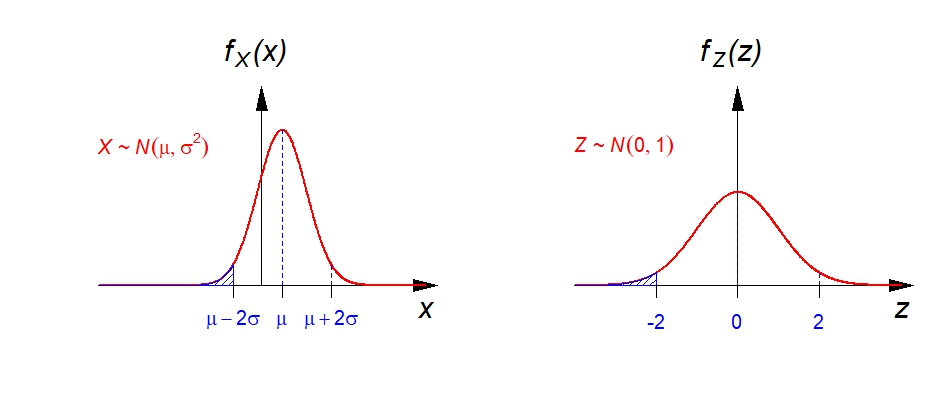
\includegraphics[width=\textwidth]{figures/04-Random_variable_probability_distribution/Normal.jpeg}
        \caption{常態分布（左）與標準常態分布（右）的機率密度函數}
        \label{fig:normal}
    \end{figure}

    \medskip

    在所有的常態分布中，我們稱平均值$\mu =0$、變異數 $\sigma^2 = 1$的常態分布為\textit{標準常態分布} (standard normal distribution)，其機率密度函數如圖\ref{fig:normal}右方所示。標準常態分布對應的隨機變數通常記為 $\ZZ$，機率密度函數則記為
    \smallskip
    \[\phi(x)=\frac{1}{\sqrt{2\pi}}e^{-\frac{x^2}{2}}\]
    \smallskip
    更重要的是，標準常態分布的累積分配函數常記為
    \smallskip
    \[\Phi(x)=\int_{-\infty}^x \frac{1}{\sqrt{2\pi}}e^{-\frac{x^2}{2}} dx\]
    \smallskip
    這個積分式只能用數值方法求值，但因為它十分重要，所以一般都會為這個函數製表，被稱為\href{https://en.wikipedia.org/wiki/Standard_normal_table}{標準常態表} (standard normal table) 或 Z 表 (Z table)。例如我們想知道 $\ZZ \ge 1.96$ 的機率，則因為常態分布是對稱的，$\ZZ \ge 1.96$ 的機率就等於 $\ZZ \le -1.96$ 的機率，查表得 $0.02500$。

    \medskip
    
    標準常態分佈重要的原因在於，任何常態分布的隨機變數在經過 \textit{z轉換} (z-transform) 後都會變成標準常態分布。換言之，若 $X \sim \NN(\mu, \sigma^2)$，則
    \smallskip
    \[\frac{X-\mu}{\sigma} \sim \NN(0,1)\]
    \smallskip
    因此，\textit{任何}常態分布的曲線下面積也都可以藉由 z 轉換求得：如果我們想知道 $X \ge x$ 的機率，那麼我們可以先算出 $x$ 經過 z 轉換後得到的 \textit{z 分數} (z-score)：
    \smallskip
    \[z = \frac{x-\mu}{\sigma}\]
    \smallskip
    此時，我們有
    \smallskip
    \[\PP(X \ge x) = \PP\Big(\frac{X-\mu}{\sigma} \ge \frac{x-\mu}{\sigma}\Big) = \PP(\ZZ \ge z)\]
    \smallskip
    所以只要在標準常態表中查詢 $\ZZ \ge z$ 的機率即可。
    
    同樣的流程可以反過來做：如果我們想知道 $X$ 取值多少以上的機率為 $\alpha$，那麼我們可以先查表找出 $\ZZ$ 取值多少以上的機率為 $\alpha$。我們把這個值記為 $z_\alpha$，也就是「對應右尾機率為 $\alpha$ 的 $z$ 值」。如此一來我們就有：
    \smallskip
    \[\alpha = \PP(\ZZ \ge z_\alpha) = \PP\Big(\frac{X-\mu}{\sigma} \ge z_\alpha \Big) = \PP(X \ge \mu + \sigma z_\alpha)\]
    \smallskip
    亦即，只要把 $z_\alpha$ 視為 z 分數做反轉換，就可以找到欲求的取值閾值。以下我們來實際動手作幾個例題：

    \medskip

    \begin{custom}{動手作}
        根據 $z_\alpha$ 的定義，$z_{0}$、$z_{1}$ 和 $z_{0.5}$ 的值應該各是多少？$z_\alpha$ 的數值應該隨著 $\alpha$ 增加而增加還是減少？另外根據 Z 表，請找出 $z_{0.025}$、$z_{0.05}$、$z_{0.975}$、$z_{0.995}$ 的數值。
    \end{custom}
    
    \medskip\noindent\framebox[\textwidth]{\rule{0pt}{250pt}}

    \bigskip

    \begin{custom}{動手作}
        假設已知清華大學的大學生身高服從一個平均值為 165 公分，標準差為 7 公分的常態分布。那麼我們預期會有多少比例的大學生身高介於 161.5 到 172 公分之間？如果我們想找出身高前 $1.5\%$ 的大學生，應該召集身高高於多少公分的學生？
    \end{custom}
    
    \medskip\noindent\framebox[\textwidth]{\rule{0pt}{250pt}}

    \bigskip

    \begin{custom}{動手作}
        在現代智力測驗中，測驗分數會根據常模轉換為平均值為 100、標準差為 15、呈現常態分布的離差智商。該常模會隨著年齡與族群不同。根據該分布，大約有多少比例的人智商會大於等於 157？如果要找出一個智商區間包含 95\% 以上的人，那麼這個智商區間是否唯一？如果並非唯一，那麼符合要求的最短智商區間應該是什麼？
    \end{custom}
    
    \medskip\noindent\framebox[\textwidth]{\rule{0pt}{250pt}}

    \bigskip

    \begin{custom}{動手作}
        根據 WHO 定義，女性之骨質密度 T 分數 (T-score) 為其骨質密度依 30-39 歲女性同部位測得之骨質密度平均值與標準差作 z 轉換後所得之值。T 分數等於或低於 -2.5 者可被診斷為骨質疏鬆。假定台灣 30-39 歲女性股骨頸骨質密度之平均值及標準差為 $0.93 \pm 0.08$ g/cm$^2$、60-69 歲女性股骨頸骨質密度之平均值及標準差為 $0.76 \pm 0.15$ g/cm$^2$。若假定女性股骨頸骨質密度之分布遵從常態分布，則理論上台灣 60-69 歲女性中，有多少比例可因股骨頸骨質密度被診斷為骨質疏鬆？
    \end{custom}

    \medskip\noindent\framebox[\textwidth]{\rule{0pt}{230pt}}

    \bigskip
    
    \begin{takehome}
        \item 機率質量函數可用來描述離散隨機變數在各數值的取值機率；機率密度函數則用來描述連續隨機變數在各數值的機率密度。
        \item 任何取值為 $0$ 或 $1$ 的二元隨機變數之分布皆可用白努利分布描述，其機率參數 $p$ 為該變數取值 $1$ 的機率。
        \item 二項分佈描述在 $n$ 次獨立二元實驗中，事件發生次數的分佈，其中每次實驗的事件發生機率為 $p$。
        \item 卜瓦松分布可描述一段時間內事件發生的次數，其平均值和變異數均為 $\lambda$。
        \item 連續隨機變數在某區間內取值的機率，等於其機率密度函數曲線在該區間下的面積。
        \item 常態分佈有兩個參數：平均值 $\mu$ 與變異數 $\sigma^2$。平均值為 $0$、變異數為 $1$ 的常態分布被稱為標準常態分布。
        \item 服從常態分佈的隨機變數可經由 z 轉換（標準化），轉換為平均數為 $0$、變異數為 $1$ 的標準常態分布。
    \end{takehome}

    \begin{docexam}{（100-1醫學(一)）}
        如果白人小孩的平均血漿醛固酮 (plasma-aldosterone) 為400 pmol/L，標準差為200 pmol/L，假設血漿醛固酮為常態分布，有多少百分比的白人小孩其血漿醛固酮$\le$ 300 pmol/L（$Pr(\ZZ \ge 0.5) = 0.3085$）？
    \end{docexam}